\documentclass[twoside]{book}

% Packages required by doxygen
\usepackage{calc}
\usepackage{doxygen}
\usepackage{graphicx}
\usepackage[utf8]{inputenc}
\usepackage{makeidx}
\usepackage{multicol}
\usepackage{multirow}
\usepackage{textcomp}
\usepackage[table]{xcolor}

% Font selection
\usepackage[T1]{fontenc}
\usepackage{mathptmx}
\usepackage[scaled=.90]{helvet}
\usepackage{courier}
\usepackage{amssymb}
\usepackage{sectsty}
\renewcommand{\familydefault}{\sfdefault}
\allsectionsfont{%
  \fontseries{bc}\selectfont%
  \color{darkgray}%
}
\renewcommand{\DoxyLabelFont}{%
  \fontseries{bc}\selectfont%
  \color{darkgray}%
}

% Page & text layout
\usepackage{geometry}
\geometry{%
  a4paper,%
  top=2.5cm,%
  bottom=2.5cm,%
  left=2.5cm,%
  right=2.5cm%
}
\tolerance=750
\hfuzz=15pt
\hbadness=750
\setlength{\emergencystretch}{15pt}
\setlength{\parindent}{0cm}
\setlength{\parskip}{0.2cm}
\makeatletter
\renewcommand{\paragraph}{%
  \@startsection{paragraph}{4}{0ex}{-1.0ex}{1.0ex}{%
    \normalfont\normalsize\bfseries\SS@parafont%
  }%
}
\renewcommand{\subparagraph}{%
  \@startsection{subparagraph}{5}{0ex}{-1.0ex}{1.0ex}{%
    \normalfont\normalsize\bfseries\SS@subparafont%
  }%
}
\makeatother

% Headers & footers
\usepackage{fancyhdr}
\pagestyle{fancyplain}
\fancyhead[LE]{\fancyplain{}{\bfseries\thepage}}
\fancyhead[CE]{\fancyplain{}{}}
\fancyhead[RE]{\fancyplain{}{\bfseries\leftmark}}
\fancyhead[LO]{\fancyplain{}{\bfseries\rightmark}}
\fancyhead[CO]{\fancyplain{}{}}
\fancyhead[RO]{\fancyplain{}{\bfseries\thepage}}
\fancyfoot[LE]{\fancyplain{}{}}
\fancyfoot[CE]{\fancyplain{}{}}
\fancyfoot[RE]{\fancyplain{}{\bfseries\scriptsize Generated on Mon Sep 5 2016 19\-:51\-:02 for Byggern by Doxygen }}
\fancyfoot[LO]{\fancyplain{}{\bfseries\scriptsize Generated on Mon Sep 5 2016 19\-:51\-:02 for Byggern by Doxygen }}
\fancyfoot[CO]{\fancyplain{}{}}
\fancyfoot[RO]{\fancyplain{}{}}
\renewcommand{\footrulewidth}{0.4pt}
\renewcommand{\chaptermark}[1]{%
  \markboth{#1}{}%
}
\renewcommand{\sectionmark}[1]{%
  \markright{\thesection\ #1}%
}

% Indices & bibliography
\usepackage{natbib}
\usepackage[titles]{tocloft}
\setcounter{tocdepth}{3}
\setcounter{secnumdepth}{5}
\makeindex

% Hyperlinks (required, but should be loaded last)
\usepackage{ifpdf}
\ifpdf
  \usepackage[pdftex,pagebackref=true]{hyperref}
\else
  \usepackage[ps2pdf,pagebackref=true]{hyperref}
\fi
\hypersetup{%
  colorlinks=true,%
  linkcolor=blue,%
  citecolor=blue,%
  unicode%
}

% Custom commands
\newcommand{\clearemptydoublepage}{%
  \newpage{\pagestyle{empty}\cleardoublepage}%
}


%===== C O N T E N T S =====

\begin{document}

% Titlepage & ToC
\hypersetup{pageanchor=false}
\pagenumbering{roman}
\begin{titlepage}
\vspace*{7cm}
\begin{center}%
{\Large Byggern }\\
\vspace*{1cm}
{\large Generated by Doxygen 1.8.6}\\
\vspace*{0.5cm}
{\small Mon Sep 5 2016 19:51:02}\\
\end{center}
\end{titlepage}
\clearemptydoublepage
\tableofcontents
\clearemptydoublepage
\pagenumbering{arabic}
\hypersetup{pageanchor=true}

%--- Begin generated contents ---
\chapter{Byggern}
\label{md__r_e_a_d_m_e}
\hypertarget{md__r_e_a_d_m_e}{}
This is the Byggern project...

This team is made up of Johan Lofstad, Sondre Baugstø and Sondre Vincent Russvoll. 



Documentation is available at \href{https://srussvoll.github.io/byggern/}{\tt https\-://srussvoll.\-github.\-io/byggern/}. 



The 'build' folder contains all build files like .hex and .elf. The 'include' folder contains all header files. The 'lib' folder contains folders with libraries containing both source and header files. The 'src' folder contains the source files. 



Added C++ support. Note that the S\-T\-L isn't implemented. More specifically, only the C standard library is available... The new and delete operators are not implemented either, so just don't use dynamic allocation without malloc(). Also remember that I\-S\-Rs are implemented in C with no support for overloading... Because of this interrupt handlers must be friends of the originator class. 
\chapter{Class Index}
\section{Class List}
Here are the classes, structs, unions and interfaces with brief descriptions\-:\begin{DoxyCompactList}
\item\contentsline{section}{\hyperlink{class_stream}{Stream} }{\pageref{class_stream}}{}
\item\contentsline{section}{\hyperlink{class_test_stream}{Test\-Stream} }{\pageref{class_test_stream}}{}
\end{DoxyCompactList}

\chapter{Class Documentation}
\hypertarget{class_u_a_r_t}{\section{U\-A\-R\-T Class Reference}
\label{class_u_a_r_t}\index{U\-A\-R\-T@{U\-A\-R\-T}}
}
Inheritance diagram for U\-A\-R\-T\-:\begin{figure}[H]
\begin{center}
\leavevmode
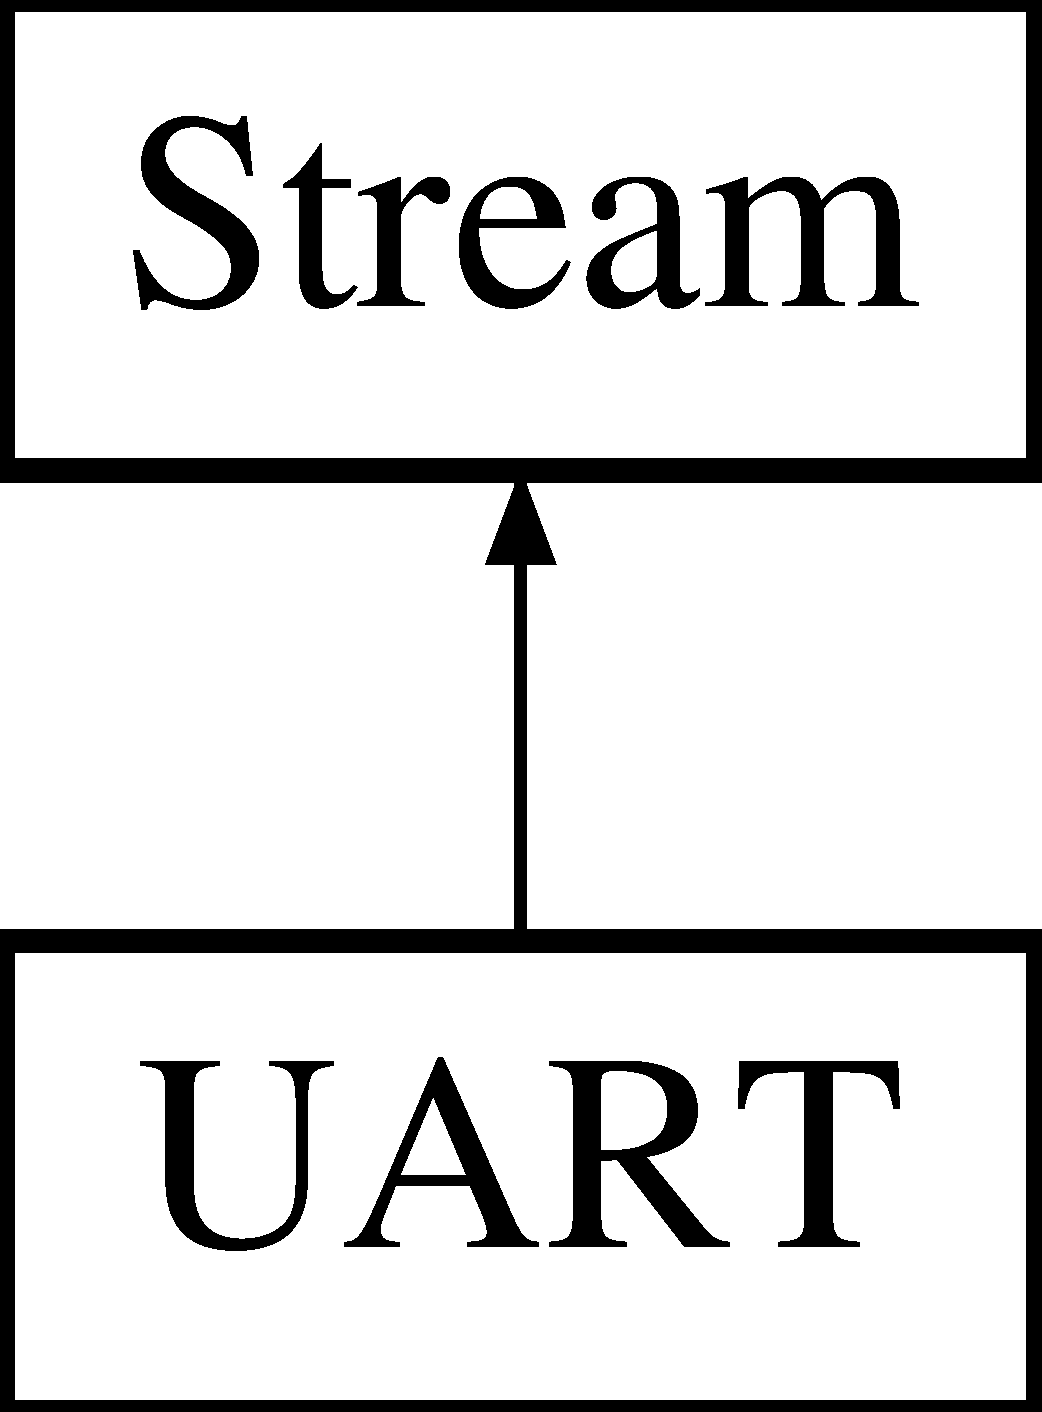
\includegraphics[height=2.000000cm]{class_u_a_r_t}
\end{center}
\end{figure}
\subsection*{Public Member Functions}
\begin{DoxyCompactItemize}
\item 
void \hyperlink{class_u_a_r_t_a8bb77ca27b4e17d608d2743313625ac4}{Write} (uint8\-\_\-t $\ast$string, uint16\-\_\-t size)
\item 
void \hyperlink{class_u_a_r_t_aed659ee8bc31ba966144d1a522506a7b}{Init} (uint16\-\_\-t baud\-\_\-rate)
\item 
\hyperlink{class_u_a_r_t_a97debffc29b178c09b104f4542298a36}{U\-A\-R\-T} (const \hyperlink{class_u_a_r_t}{U\-A\-R\-T} \&)=delete
\item 
void \hyperlink{class_u_a_r_t_a843ab7fc20f5ce5f030d2ca5ee98d6b6}{operator=} (const \hyperlink{class_u_a_r_t}{U\-A\-R\-T} \&)=delete
\end{DoxyCompactItemize}
\subsection*{Static Public Member Functions}
\begin{DoxyCompactItemize}
\item 
static \hyperlink{class_u_a_r_t}{U\-A\-R\-T} \& \hyperlink{class_u_a_r_t_a745c8f35f3ca3ab6359cedda3e640777}{Get\-Instance} ()
\end{DoxyCompactItemize}
\subsection*{Private Member Functions}
\begin{DoxyCompactItemize}
\item 
\hypertarget{class_u_a_r_t_a195cdcca08c2ae1d03ee8bf13a87b95a}{void {\bfseries initialize\-\_\-transmission} ()}\label{class_u_a_r_t_a195cdcca08c2ae1d03ee8bf13a87b95a}

\item 
\hyperlink{class_u_a_r_t_a68e7e88d2a13f5da85f0fde1ef98515f}{U\-A\-R\-T} ()
\end{DoxyCompactItemize}
\subsection*{Private Attributes}
\begin{DoxyCompactItemize}
\item 
\hypertarget{class_u_a_r_t_ae98e7d277a1833478aa85dc9e686150a}{bool {\bfseries ongoing\-\_\-transmission} = false}\label{class_u_a_r_t_ae98e7d277a1833478aa85dc9e686150a}

\end{DoxyCompactItemize}
\subsection*{Friends}
\begin{DoxyCompactItemize}
\item 
void \hyperlink{class_u_a_r_t_accc13d37cd82c841e387e1d5cf4d9a94}{U\-S\-A\-R\-T0\-\_\-\-U\-D\-R\-E\-\_\-vect} ()
\end{DoxyCompactItemize}
\subsection*{Additional Inherited Members}


\subsection{Constructor \& Destructor Documentation}
\hypertarget{class_u_a_r_t_a97debffc29b178c09b104f4542298a36}{\index{U\-A\-R\-T@{U\-A\-R\-T}!U\-A\-R\-T@{U\-A\-R\-T}}
\index{U\-A\-R\-T@{U\-A\-R\-T}!UART@{U\-A\-R\-T}}
\subsubsection[{U\-A\-R\-T}]{\setlength{\rightskip}{0pt plus 5cm}U\-A\-R\-T\-::\-U\-A\-R\-T (
\begin{DoxyParamCaption}
\item[{const {\bf U\-A\-R\-T} \&}]{}
\end{DoxyParamCaption}
)\hspace{0.3cm}{\ttfamily [delete]}}}\label{class_u_a_r_t_a97debffc29b178c09b104f4542298a36}
Beacause of singleton -\/ makes sure its not copied etc. \hypertarget{class_u_a_r_t_a68e7e88d2a13f5da85f0fde1ef98515f}{\index{U\-A\-R\-T@{U\-A\-R\-T}!U\-A\-R\-T@{U\-A\-R\-T}}
\index{U\-A\-R\-T@{U\-A\-R\-T}!UART@{U\-A\-R\-T}}
\subsubsection[{U\-A\-R\-T}]{\setlength{\rightskip}{0pt plus 5cm}U\-A\-R\-T\-::\-U\-A\-R\-T (
\begin{DoxyParamCaption}
{}
\end{DoxyParamCaption}
)\hspace{0.3cm}{\ttfamily [private]}}}\label{class_u_a_r_t_a68e7e88d2a13f5da85f0fde1ef98515f}
A constructor that initializes the \hyperlink{class_u_a_r_t}{U\-A\-R\-T} to a certain size 

\subsection{Member Function Documentation}
\hypertarget{class_u_a_r_t_a745c8f35f3ca3ab6359cedda3e640777}{\index{U\-A\-R\-T@{U\-A\-R\-T}!Get\-Instance@{Get\-Instance}}
\index{Get\-Instance@{Get\-Instance}!UART@{U\-A\-R\-T}}
\subsubsection[{Get\-Instance}]{\setlength{\rightskip}{0pt plus 5cm}static {\bf U\-A\-R\-T}\& U\-A\-R\-T\-::\-Get\-Instance (
\begin{DoxyParamCaption}
{}
\end{DoxyParamCaption}
)\hspace{0.3cm}{\ttfamily [inline]}, {\ttfamily [static]}}}\label{class_u_a_r_t_a745c8f35f3ca3ab6359cedda3e640777}
A Singleton implementation of this class \hypertarget{class_u_a_r_t_aed659ee8bc31ba966144d1a522506a7b}{\index{U\-A\-R\-T@{U\-A\-R\-T}!Init@{Init}}
\index{Init@{Init}!UART@{U\-A\-R\-T}}
\subsubsection[{Init}]{\setlength{\rightskip}{0pt plus 5cm}void U\-A\-R\-T\-::\-Init (
\begin{DoxyParamCaption}
\item[{uint16\-\_\-t}]{baud\-\_\-rate}
\end{DoxyParamCaption}
)}}\label{class_u_a_r_t_aed659ee8bc31ba966144d1a522506a7b}
Initializer because of the singleton implementation. 
\begin{DoxyParams}{Parameters}
{\em baud\-\_\-rate} & The baud rate of the uart \\
\hline
\end{DoxyParams}
\hypertarget{class_u_a_r_t_a843ab7fc20f5ce5f030d2ca5ee98d6b6}{\index{U\-A\-R\-T@{U\-A\-R\-T}!operator=@{operator=}}
\index{operator=@{operator=}!UART@{U\-A\-R\-T}}
\subsubsection[{operator=}]{\setlength{\rightskip}{0pt plus 5cm}void U\-A\-R\-T\-::operator= (
\begin{DoxyParamCaption}
\item[{const {\bf U\-A\-R\-T} \&}]{}
\end{DoxyParamCaption}
)\hspace{0.3cm}{\ttfamily [delete]}}}\label{class_u_a_r_t_a843ab7fc20f5ce5f030d2ca5ee98d6b6}
Beacause of singleton -\/ makes sure its not copied etc. \hypertarget{class_u_a_r_t_a8bb77ca27b4e17d608d2743313625ac4}{\index{U\-A\-R\-T@{U\-A\-R\-T}!Write@{Write}}
\index{Write@{Write}!UART@{U\-A\-R\-T}}
\subsubsection[{Write}]{\setlength{\rightskip}{0pt plus 5cm}void U\-A\-R\-T\-::\-Write (
\begin{DoxyParamCaption}
\item[{uint8\-\_\-t $\ast$}]{string, }
\item[{uint16\-\_\-t}]{size}
\end{DoxyParamCaption}
)\hspace{0.3cm}{\ttfamily [virtual]}}}\label{class_u_a_r_t_a8bb77ca27b4e17d608d2743313625ac4}
Write the inserted string to output (i.\-e. write to computer) 
\begin{DoxyParams}{Parameters}
{\em string} & The \char`\"{}data string\char`\"{} that shall be written to the output \\
\hline
{\em size} & the size of the data string \\
\hline
\end{DoxyParams}


Reimplemented from \hyperlink{class_stream_a508be3423e4d99ab2757275fb723002a}{Stream}.



\subsection{Friends And Related Function Documentation}
\hypertarget{class_u_a_r_t_accc13d37cd82c841e387e1d5cf4d9a94}{\index{U\-A\-R\-T@{U\-A\-R\-T}!U\-S\-A\-R\-T0\-\_\-\-U\-D\-R\-E\-\_\-vect@{U\-S\-A\-R\-T0\-\_\-\-U\-D\-R\-E\-\_\-vect}}
\index{U\-S\-A\-R\-T0\-\_\-\-U\-D\-R\-E\-\_\-vect@{U\-S\-A\-R\-T0\-\_\-\-U\-D\-R\-E\-\_\-vect}!UART@{U\-A\-R\-T}}
\subsubsection[{U\-S\-A\-R\-T0\-\_\-\-U\-D\-R\-E\-\_\-vect}]{\setlength{\rightskip}{0pt plus 5cm}void U\-S\-A\-R\-T0\-\_\-\-U\-D\-R\-E\-\_\-vect (
\begin{DoxyParamCaption}
{}
\end{DoxyParamCaption}
)\hspace{0.3cm}{\ttfamily [friend]}}}\label{class_u_a_r_t_accc13d37cd82c841e387e1d5cf4d9a94}
The interrupt handler vector. To be run on each D\-R\-E interrupt 

The documentation for this class was generated from the following files\-:\begin{DoxyCompactItemize}
\item 
lib/uart/\hyperlink{uart_8h}{uart.\-h}\item 
lib/uart/uart.\-cpp\end{DoxyCompactItemize}

\hypertarget{struct_u_a_r_t_registers}{\section{U\-A\-R\-T\-Registers Struct Reference}
\label{struct_u_a_r_t_registers}\index{U\-A\-R\-T\-Registers@{U\-A\-R\-T\-Registers}}
}
\subsection*{Public Attributes}
\begin{DoxyCompactItemize}
\item 
\hypertarget{struct_u_a_r_t_registers_a319ffcce39d3a759f8b8f99caeffd6ff}{volatile uint8\-\_\-t $\ast$ {\bfseries U\-D\-R}}\label{struct_u_a_r_t_registers_a319ffcce39d3a759f8b8f99caeffd6ff}

\item 
\hypertarget{struct_u_a_r_t_registers_a5617be018643b8bbf302e9e7f0574662}{volatile uint8\-\_\-t $\ast$ {\bfseries U\-C\-S\-R\-A}}\label{struct_u_a_r_t_registers_a5617be018643b8bbf302e9e7f0574662}

\item 
\hypertarget{struct_u_a_r_t_registers_aa9d53e58476eb92a89921a9cc4542a80}{volatile uint8\-\_\-t $\ast$ {\bfseries U\-C\-S\-R\-B}}\label{struct_u_a_r_t_registers_aa9d53e58476eb92a89921a9cc4542a80}

\item 
\hypertarget{struct_u_a_r_t_registers_ad066bd333b8f00ad809db7fbefa9364f}{volatile uint8\-\_\-t $\ast$ {\bfseries U\-C\-S\-R\-C}}\label{struct_u_a_r_t_registers_ad066bd333b8f00ad809db7fbefa9364f}

\item 
\hypertarget{struct_u_a_r_t_registers_a71e0561ae6d0d0f7aeb21c112aeb1c26}{volatile uint8\-\_\-t $\ast$ {\bfseries U\-B\-R\-R\-L}}\label{struct_u_a_r_t_registers_a71e0561ae6d0d0f7aeb21c112aeb1c26}

\item 
\hypertarget{struct_u_a_r_t_registers_ae39abc442e09526eed2493efdb80279a}{volatile uint8\-\_\-t $\ast$ {\bfseries U\-B\-R\-R\-H}}\label{struct_u_a_r_t_registers_ae39abc442e09526eed2493efdb80279a}

\end{DoxyCompactItemize}


The documentation for this struct was generated from the following file\-:\begin{DoxyCompactItemize}
\item 
lib/uart/U\-A\-R\-T.\-h\end{DoxyCompactItemize}

%--- End generated contents ---

% Index
\newpage
\phantomsection
\addcontentsline{toc}{chapter}{Index}
\printindex

\end{document}
